% Options for packages loaded elsewhere
\PassOptionsToPackage{unicode}{hyperref}
\PassOptionsToPackage{hyphens}{url}
%
\documentclass[
  ignorenonframetext,
]{beamer}
\usepackage{pgfpages}
\setbeamertemplate{caption}[numbered]
\setbeamertemplate{caption label separator}{: }
\setbeamercolor{caption name}{fg=normal text.fg}
\beamertemplatenavigationsymbolsempty
% Prevent slide breaks in the middle of a paragraph
\widowpenalties 1 10000
\raggedbottom
\setbeamertemplate{part page}{
  \centering
  \begin{beamercolorbox}[sep=16pt,center]{part title}
    \usebeamerfont{part title}\insertpart\par
  \end{beamercolorbox}
}
\setbeamertemplate{section page}{
  \centering
  \begin{beamercolorbox}[sep=12pt,center]{part title}
    \usebeamerfont{section title}\insertsection\par
  \end{beamercolorbox}
}
\setbeamertemplate{subsection page}{
  \centering
  \begin{beamercolorbox}[sep=8pt,center]{part title}
    \usebeamerfont{subsection title}\insertsubsection\par
  \end{beamercolorbox}
}
\AtBeginPart{
  \frame{\partpage}
}
\AtBeginSection{
  \ifbibliography
  \else
    \frame{\sectionpage}
  \fi
}
\AtBeginSubsection{
  \frame{\subsectionpage}
}
\usepackage{lmodern}
\usepackage{amsmath}
\usepackage{ifxetex,ifluatex}
\ifnum 0\ifxetex 1\fi\ifluatex 1\fi=0 % if pdftex
  \usepackage[T1]{fontenc}
  \usepackage[utf8]{inputenc}
  \usepackage{textcomp} % provide euro and other symbols
  \usepackage{amssymb}
\else % if luatex or xetex
  \usepackage{unicode-math}
  \defaultfontfeatures{Scale=MatchLowercase}
  \defaultfontfeatures[\rmfamily]{Ligatures=TeX,Scale=1}
\fi
% Use upquote if available, for straight quotes in verbatim environments
\IfFileExists{upquote.sty}{\usepackage{upquote}}{}
\IfFileExists{microtype.sty}{% use microtype if available
  \usepackage[]{microtype}
  \UseMicrotypeSet[protrusion]{basicmath} % disable protrusion for tt fonts
}{}
\makeatletter
\@ifundefined{KOMAClassName}{% if non-KOMA class
  \IfFileExists{parskip.sty}{%
    \usepackage{parskip}
  }{% else
    \setlength{\parindent}{0pt}
    \setlength{\parskip}{6pt plus 2pt minus 1pt}}
}{% if KOMA class
  \KOMAoptions{parskip=half}}
\makeatother
\usepackage{xcolor}
\IfFileExists{xurl.sty}{\usepackage{xurl}}{} % add URL line breaks if available
\IfFileExists{bookmark.sty}{\usepackage{bookmark}}{\usepackage{hyperref}}
\hypersetup{
  pdftitle={What Teachers Value About Online PD},
  pdfauthor={Shaun Kellogg},
  hidelinks,
  pdfcreator={LaTeX via pandoc}}
\urlstyle{same} % disable monospaced font for URLs
\newif\ifbibliography
\usepackage{graphicx}
\makeatletter
\def\maxwidth{\ifdim\Gin@nat@width>\linewidth\linewidth\else\Gin@nat@width\fi}
\def\maxheight{\ifdim\Gin@nat@height>\textheight\textheight\else\Gin@nat@height\fi}
\makeatother
% Scale images if necessary, so that they will not overflow the page
% margins by default, and it is still possible to overwrite the defaults
% using explicit options in \includegraphics[width, height, ...]{}
\setkeys{Gin}{width=\maxwidth,height=\maxheight,keepaspectratio}
% Set default figure placement to htbp
\makeatletter
\def\fps@figure{htbp}
\makeatother
\setlength{\emergencystretch}{3em} % prevent overfull lines
\providecommand{\tightlist}{%
  \setlength{\itemsep}{0pt}\setlength{\parskip}{0pt}}
\setcounter{secnumdepth}{-\maxdimen} % remove section numbering
\ifluatex
  \usepackage{selnolig}  % disable illegal ligatures
\fi

\title{What Teachers Value About Online PD}
\subtitle{A Text Analysis of Open-Ended Survey Reponses}
\author{Shaun Kellogg}
\date{February 9, 2021}

\begin{document}
\frame{\titlepage}

\begin{frame}{Questions}
\protect\hypertarget{questions}{}
\begin{enumerate}
\item
  What aspects of online professional learning resources do teachers
  find most valuable?
\item
  How might online learning resources differ in the value they afford
  teachers?
\end{enumerate}
\end{frame}

\begin{frame}{Methods}
\protect\hypertarget{methods}{}
\textbf{Data Source}: Items pertaining educator role, resource type, and
value of resource on RttT Online Resources Survey

\textbf{Data Processing}: Tokenized and tidied text

\textbf{Data Analysis}: Word Counts \& Term Frequency-Inverse Document
Frequency
\end{frame}

\hypertarget{findings}{%
\section{Findings}\label{findings}}

\begin{frame}{Words Used to Describe Benefits}
\protect\hypertarget{words-used-to-describe-benefits}{}

\includegraphics[width=0.75\textwidth,height=\textheight]{img/cloud-clean.png}
\end{frame}

\begin{frame}{Top 20 Words}
\protect\hypertarget{top-20-words}{}
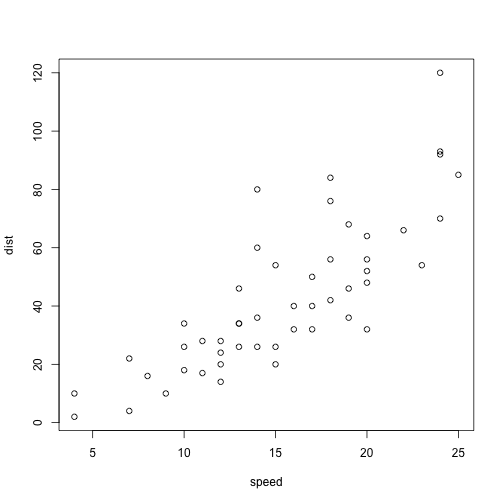
\includegraphics{unit-1-product_files/figure-beamer/unnamed-chunk-3-1.pdf}
\end{frame}

\begin{frame}{Information Shared}
\protect\hypertarget{information-shared}{}
``It could be completed at home in my free time. It had lots of good
information that helped me understand the \textbf{terminology}.''

``the information about the way our \textbf{common core} was created for
our system''

``Informative information on the \textbf{21st century learner} and
teacher.''

``The most beneficial aspect was the information about \textbf{types of
data} and where we get it from.''

``This has already been implemented; I do not need to know this
information at this point.''
\end{frame}

\begin{frame}{Videos and Resource Provided}
\protect\hypertarget{videos-and-resource-provided}{}
``All the videos and resources''

``\textbf{Printable resources} to keep on hand and example videos of how
to use formative assessments in the classroom.''

``I was able to see other \textbf{lesson plans} and resources that other
schools are doing.''

``Viewing \textbf{teacher videos}, especially Dan Meyer and Finland
classroom. I was also introduced to new online resources that will aid
my students and me in learning.''

``This was not a beneficial resource to me as I do not teach nor will
grade the MSLs for the subject areas targeted in this resource.''
\end{frame}

\begin{frame}{Time and Pace for Learning}
\protect\hypertarget{time-and-pace-for-learning}{}
``The \textbf{ability to schedule the time to work} on the module so
that it does not interfere with my commitments as an educator.''

``time to \textbf{talk with peers}''

``The most valuable aspect was the time factor. This online module was
my first. I did not realize I could \textbf{walk away and work on it at
another time}, so this is a tremendous aspect for the online learner.''

``Teachers are \textbf{able to go back to the information at anytime} to
view the information to ensure understanding of the material.''

``The \textbf{freedom} to work at my own pace.''
\end{frame}

\begin{frame}{Words Emphasized in Each Resource}
\protect\hypertarget{words-emphasized-in-each-resource}{}
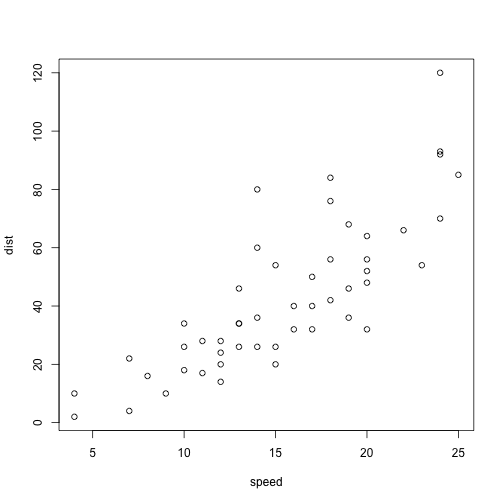
\includegraphics{unit-1-product_files/figure-beamer/unnamed-chunk-7-1.pdf}
\end{frame}

\begin{frame}{Conclusions}
\protect\hypertarget{conclusions}{}
\begin{enumerate}
\tightlist
\item
  Teachers found the \textbf{information} shared beneficial, such as new
  terminology, the common core standards, and types of data.
\item
  Teachers appreciated the \textbf{resources and videos} provided
  including lesson plans and printable materials.
\item
  A broad theme to emerge was the \textbf{convenience} of online
  professional development with respect to time, pace, and format.
\end{enumerate}
\end{frame}

\begin{frame}{Discussion}
\protect\hypertarget{discussion}{}
\begin{itemize}
\tightlist
\item
  \textbf{Limitations}: While able to provide quick insight into a large
  number of responses, analysis raised as many questions as it
  answered.\\
\item
  \textbf{Implications}: Validation of design decisions such use of
  videos and inclusion of practical resources.\\
\item
  \textbf{Next Steps for Analysis}: Dig into recommendations for
  improvement.
\end{itemize}
\end{frame}

\end{document}
